\documentclass[mathserif]{beamer}
\usepackage[utf8]{inputenc}
\usepackage[T1]{fontenc}
\usepackage[ngerman,german]{babel}
\usepackage{amsmath}
\usepackage{amsthm}
\usepackage{amssymb}
\usepackage{tikz}
\usepackage{bbold}
\usepackage{enumerate}
\usepackage{ifthen}
\usepackage{breqn}
\usepackage{floatrow}
\usetikzlibrary{shapes,shadows,arrows,decorations.markings}
\usetikzlibrary{decorations.pathreplacing,calc}
\usetheme{Szeged}
\usecolortheme{seagull}

\newcommand{\inftyint}{\int_{-\infty}^{\infty}}
\newcommand{\intR}{\int_{\mathbb{R}}}
\newcommand{\intRRR}{\int_{\mathbb{R}^3}}
\newcommand{\opd}[2][\vphantom{1}]{\!\operatorname{d}^{#1}\! #2\ }
\newcommand{\opdpath}{\opd{\mu(p)}}
\newcommand{\real}{\operatorname{Re}}
\newcommand{\imag}{\operatorname{Im}}
\newcommand{\residue}{\operatorname{Res}}
\newcommand{\veps}{\varepsilon}
\newcommand{\vx}{\vec{x}}
\newcommand{\vp}{\vec{p}}
\newcommand{\vacuumt}{\langle 0 |}
\newcommand{\vacuum}{| 0 \rangle}
\newcommand{\Res}{\operatorname{Res}}
\newcommand{\inHS}{{}^{(3)}\!}
\newcommand{\VSthree}{\mu(\mathcal{S}^3)}

\title{\textbf{Das Problem der Zeit in der Quantengravitation}}
\author{\small {Teil 1: Vorbereitungen und allgemeine Betrachtungen}}
\institute{}
\date{\today}

\theoremstyle{definition}

\begin{document}
	\begin{frame}
		\titlepage
	\end{frame}

	\begin{frame}{Überblick}
		\tableofcontents
	\end{frame}

\section{Mathematische Konzepte der Differentialgeometrie}
\begin{frame}
\begin{center}
	\large \textbf{Mathematische Konzepte der Differentialgeometrie}
\end{center}
\end{frame}
\subsection{Mannigfaltigkeiten}
	\begin{frame}{Mannigfaltigkeit}
		Eine n-dimensionale Mannigfaltigkeit ist Menge $M$, die lokal die selbe Struktur wie $\mathbb{R}^n$.\\
		
			Beispiel:
			
		\pause
		\begin{minipage}{0.45\linewidth}
			
			\centering
			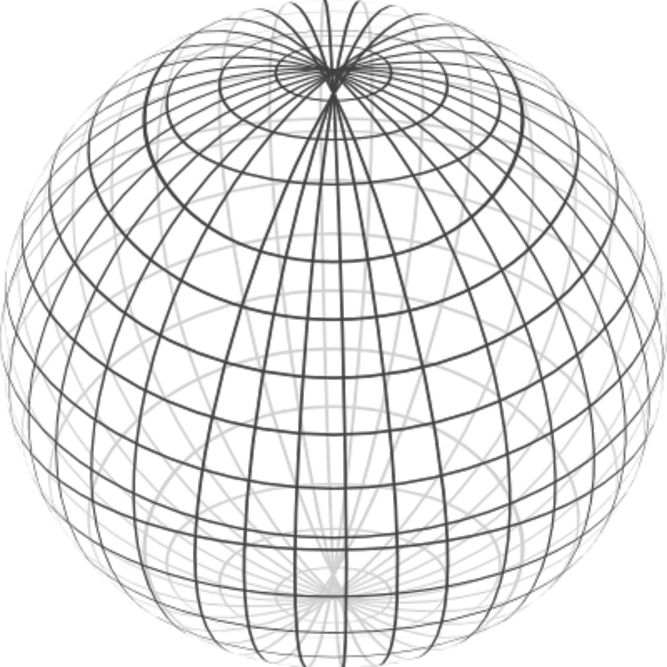
\includegraphics[scale=0.3]{sphere.pdf}
		\end{minipage}
		\hfill
		\pause
		\begin{minipage}{0.45\linewidth}
			
			\centering
			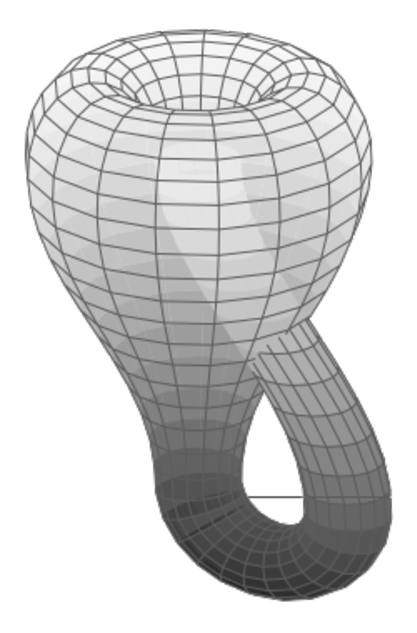
\includegraphics[scale=0.3]{bottle.pdf}
		\end{minipage}\\
		\begin{itemize}
			\item $M$ Teilmenge eines h\"oherdimensionalen Raumes mit Dimension $m$:\\
			$M$ is eingebettet.\\
			\pause
			\item Dimension von $M$ gleich $m-1$:\\
			$M$ ist eine Hyperebene
		\end{itemize}
	\end{frame}
\subsection{Metrik}
	\begin{frame}{Metrik}
		allgemeine Formulierung für einen Distanzbegriff\\
		Entfernung zwischen zwei Punkten hängt von der ,,Form`` ab.\\
		\pause
		$\rightarrow$ Charakterisierung mittels Metriktensors $g$:
		\begin{align}
			{\rm d}s^2=g_{\mu\nu}{\rm d}x^\mu{\rm d}x^\nu
		\end{align}\\
		Länge einer Kurve:
		\begin{align}
			\int {\rm d}s=\int_{t_1}^{t_2}{\rm d}t\, \sqrt{g_{\mu\nu}{\rm d}x(t)^\mu{\rm d}x(t)^\nu}
		\end{align}
	\end{frame}
	
	\begin{frame}
		Beispiel: Zylinder\\
		\begin{center}
			


\begin{tikzpicture}[y=0.80pt, x=0.8pt,yscale=-1, inner sep=0pt, outer sep=0pt]
\begin{scope}[shift={(-69.44543,-862.60218)}]
  \path[cm={{0.86136,-0.508,0.508,0.86136,(-435.02941,302.9781)}},draw=black,line
    join=miter,line cap=butt,miter limit=4.00,line width=0.400pt]
    (410.0000,895.4872) .. controls (410.0000,905.4973) and (377.5406,913.6122) ..
    (337.5000,913.6122) .. controls (297.4594,913.6122) and (265.0000,905.4973) ..
    (265.0000,895.4872) .. controls (265.0000,885.4770) and (297.4594,877.3622) ..
    (337.5000,877.3622) .. controls (377.5406,877.3622) and (410.0000,885.4770) ..
    (410.0000,895.4872) -- cycle;
  \path[draw=black,line join=miter,line cap=butt,miter limit=4.00,line
    width=0.400pt] (249.0882,941.3095) -- (302.4279,1031.7522);
  \path[draw=black,line join=miter,line cap=butt,miter limit=4.00,line
    width=0.400pt] (373.9569,867.3734) -- (427.2966,957.8160);
  \path[draw=black,line join=miter,line cap=butt,miter limit=4.00,line
    width=0.400pt] (426.8804,957.3389) .. controls (431.9655,965.9612) and
    (408.1287,989.4403) .. (373.6393,1009.7808) .. controls (339.1500,1030.1213)
    and (307.0685,1039.6208) .. (301.9834,1030.9985);
  \path[draw=black,dash pattern=on 3.20pt off 1.60pt,line join=miter,line
    cap=butt,miter limit=4.00,line width=0.400pt] (426.9439,957.4466) .. controls
    (421.8588,948.8242) and (389.7773,958.3237) .. (355.2880,978.6642) .. controls
    (320.7986,999.0048) and (296.9618,1022.4838) .. (302.0469,1031.1062);
  \path[draw=black,miter limit=4.00,line width=0.400pt,rounded corners=0.0000cm]
    (69.6954,958.1198) rectangle (172.3740,1044.7269);
  \path[draw=black,fill=black,miter limit=4.00,line width=0.800pt]
    (85.9321,965.9745) -- (82.8610,967.9948) -- (85.9321,960.9237) --
    (89.0032,967.9948) -- cycle;
  \path[draw=black,line join=miter,line cap=butt,miter limit=4.00,line
    width=0.400pt] (85.9892,966.6255) -- (85.9892,1040.9980);
  \path[draw=black,line join=miter,line cap=butt,miter limit=4.00,line
    width=0.400pt] (74.1199,1029.7600) -- (156.9524,1029.7600);
  \path[draw=black,fill=black,miter limit=4.00,line width=0.800pt]
    (157.3312,1029.7600) -- (155.3109,1026.6889) -- (162.3820,1029.7600) --
    (155.3109,1032.8310) -- cycle;
  \path[draw=black,line join=miter,line cap=butt,line width=0.800pt]
    (126.2691,952.3571) .. controls (165.9766,870.8115) and (191.3674,1010.4302)
    .. (262.6397,988.7226);
  \path[draw=black,fill=black,miter limit=4.00,line width=0.800pt]
    (263.0056,988.4181) -- (260.0930,986.1753) -- (267.7794,986.7684) --
    (262.0992,991.9806) -- cycle;
  \path[fill=black] (93.186569,974.58044) node[above right] (text3863) {$z$};
  \path[fill=black] (148.99751,1019.7849) node[above right] (text3867) {$\phi$};
  \path[fill=black] (165.66502,928.61853) node[above right] (text3871)
    {$\vec{x}(\phi,z)$};
\end{scope}

\end{tikzpicture}

		\end{center}
		Metriktensor f\"ur diese Beispiel: $g=\left(\begin{array}{cc} r & 0 \\ 0 & 1 \end{array}\right)$
	\end{frame}
\subsection{Kovariante Ableitung}
	\begin{frame}{Kovariante Ableitung}
		Betrachten Ableitungsbegriff für eingebettete Ebenen in $\mathbb{R}^3$:
		\begin{itemize}
		\item Benötigen Differentiatonsbegriff, der die Deformiertheit der Mannigfaltigkeit berücksichtigt.\\
		\pause
		\item Für Skalarfelder ist die klassische Definition ausreichend.\\
		Für Vektoren und Tensore aber nicht!$\rightarrow$ Wollen, dass Ableitung ,,nur in der Ebene wirkt``\\
		\pause
		\end{itemize}
	\end{frame}
	\begin{frame}
		Tangentialraum ($T_p(M)$): Vektorraum an jede Punkt der Mannigfaltigkeit
		\begin{itemize}
			\item Für eindimensionale Kurve: Alle vielfache des Tangentenvektors
			\item Für Fläche: Linearkombinationen von 2 Tangentenvektoren
		\end{itemize}
		\pause
		Wir wollen mit der Ableitung sozusagen nicht aus dem Tangentialraum ausbrechen:
		\begin{center}
		$\rightarrow$ Wähle Projektion der normalen Ableitung
		\end{center}
	\end{frame}
	\begin{frame}
		Situation für zweidimensionale Riemannsche Mannigfaltigkeiten:
		\begin{itemize}
			\item Ableiten eines Vektors $v=a \vx_u+b\vx_v$ entlang Kurve
			\pause
			\item Identifzieren der Vektoren $\vx_{uu},\ \vx_{uv}$ und $\vx_{vv}$:
				\begin{align*}
					\vec{x}_{uu}&=\Gamma^1_{11} \vx_u+\Gamma^2_{11}\vx_v+L_1 n\\
					\vx_{uv}&=\Gamma^1_{12}\vx_u+\Gamma^2_{12}\vx_v +L_2 n\\
					\vx_{vv}&=\Gamma^1_{22}\vx_u+\Gamma^2_{22}\vx_v+L_3 n
				\end{align*}
			\pause
			\item In Ableitung einsetzen
		\end{itemize}
	\end{frame}
	
	\begin{frame}
		Ignorieren der Normalkomponenten:
		\begin{align*}
			\frac{{\rm D} v(t)}{{\rm d}t}=\nabla_{v(t)} v(t) :=& (\dot{a} + \Gamma^1_{11}a^2+\Gamma^1_{12}ab+\Gamma^1_{22}b^2)\vx_u+\notag\\
			+&(\dot{b} + \Gamma^2_{11}a^2+\Gamma^2_{12}ab+\Gamma^2_{22}b^2)\vx_v.
		\end{align*}
		\pause
		oder in kompakter Notation mit Koorinatenachsen als Ableitungsrichtungen:
		\begin{align*}
			\nabla_\mu v^\nu=\partial_\mu v^\nu +\Gamma^\nu_{\rho\mu}v^\rho.
		\end{align*}
		\pause
		Christoffelsymbole: $\Gamma^\mu_{\nu\rho}=\frac{1}{2}g^{\mu\sigma}(\partial_\rho g_{\sigma \nu}+\partial_\nu g_{\sigma \rho}-\partial_\sigma g_{\nu\rho})$
	\end{frame}
\subsection{Krümmung}
	\begin{frame}{Krümmung}
		Zwei zentrale Begriffe:
		\begin{itemize}
			\item \textbf{Intrinsische Krümmung}:\\
				Unabhängig vom Einbettungsraum -- Zylinder hat die selbe intrinsische Krümmung wie eine Fläche
			\pause
			\item \textbf{Extrinisische Krümmung}:\\
				Abhängig von der Wahl der Einbettung -- Zylinder ist gekrümmmte Fläche im $\mathbb{R}^3$, aber einfache Fläche nicht
		\end{itemize}
	\end{frame}
	\begin{frame}{Krümmung}
		Zwei zentrale Begriffe:
		\begin{itemize}
			\item \textbf{Intrinsische Krümmung}:\\
				Angegeben über $R^\rho{}_{\sigma\mu\nu}\ \rightarrow$ Riemannscher Krümmungstensor
			\item \textbf{Extrinisische Krümmung}:\\
				intuitiv: ,,Wie stark ändert sich ein Normalenvektor $n$ in einer Umgebung um einen Punkt``
			\begin{center}
				$n$ existiert \textit{nur}, wenn die Manigfaltigkeit eingebettet ist!
			\end{center}
		\end{itemize}
	\end{frame}
	\begin{frame}
		\textbf{Intrinsische Krümmung}:\\
				Lässt sich über die (intrinsischen) Christoffelsymbole angeben:
				\begin{align}
					R^\rho{}_{\sigma\mu\nu} = \partial_\mu\Gamma^\rho{}_{\nu\sigma}
						- \partial_\nu\Gamma^\rho{}_{\mu\sigma}
						+ \Gamma^\rho{}_{\mu\lambda}\Gamma^\lambda{}_{\nu\sigma}
						- \Gamma^\rho{}_{\nu\lambda}\Gamma^\lambda{}_{\mu\sigma}
				\end{align}
				Keine Beteiligung von einbettungsbezogenen Größen (wie etwa Normalvektoren!)
	\end{frame}
	\begin{frame}
		\textbf{Extrinisische Krümmung}:\\
				Definiert auf Hyperebenen mit Normalvektor $n$:
				\begin{definition} Extrinisische Krümmung K:
					\begin{align}
						K:\ T_p(\Sigma)\times T_p(\Sigma)&\rightarrow \mathbb{R} \label{def:extrcurv} \\
							(v,u)&\mapsto -\langle v,L(u)\rangle.\notag
					\end{align}
				\end{definition}
				Wobei
				\begin{align*}
					L:\ T_p(\Sigma)&\rightarrow T_p(\Sigma) \\
						v&\mapsto \nabla_v n
				\end{align*}
				die Weingartenabbildung bezeichnet.
	\end{frame}
	\begin{frame}
		\textbf{Extrinisische Krümmung}:\\
				\begin{center}
					


\begin{tikzpicture}[y=0.80pt, x=0.8pt,yscale=-1, inner sep=0pt, outer sep=0pt]
  \path[draw=black,line join=miter,line cap=butt,line width=0.800pt]
    (87.8571,893.7908) .. controls (155.0347,690.4082) and (299.3718,975.1572) ..
    (374.2857,768.7908);
  \path[draw=black,line join=miter,line cap=butt,line width=0.800pt]
    (298.9286,848.0765) -- (295.7143,809.3265);
  \path[fill=black] (294.8553,805.4567) -- (298.1777,811.2726) --
    (295.6293,809.9772) -- (293.6572,812.0466) -- cycle;
  \path[fill=black] (300.34708,828.74585) node[above right] (text3045) {$n$};
  \path[draw=black,line join=miter,line cap=butt,miter limit=4.00,line
    width=0.299pt] (294.6134,805.6502) -- (268.1114,807.8485);
  \path[fill=black,miter limit=4.00,line width=0.320pt] (263.9260,808.5841) --
    (269.7419,805.2618) -- (268.4465,807.8101) -- (270.5159,809.7823) -- cycle;
  \path[fill=black] (264.90817,802.41815) node[above right] (text3840) {$\nabla_v
    n$};
  \path[draw=black,line join=miter,line cap=butt,line width=0.800pt]
    (299.6187,847.9412) -- (216.9401,855.8127);
  \path[fill=black] (212.8025,856.6287) -- (218.6184,853.3064) --
    (217.3230,855.8547) -- (219.3924,857.8269) -- cycle;
  \path[draw=black,dash pattern=on 0.80pt off 0.80pt,line join=miter,line
    cap=butt,miter limit=4.00,line width=0.800pt] (382.0132,840.0824) --
    (299.3347,847.9540);
  \path[fill=black] (210.71428,852.36218) node[above right] (text3866) {$v$};

\end{tikzpicture}

				\end{center}
	\end{frame}
	\begin{frame}
		Zusammenhang zwischen Größen der Hyperebene und des Umgebungsraumes:
		\begin{center}
			\textbf{Gauss-Codazzi Gleichung:}
		\end{center}
		\begin{align}
			{P^\mu}_\alpha{P^\nu}_\beta{P^\gamma}_\rho{P^\sigma}_\delta {R^\rho}_{\sigma\mu\nu}={\inHS R^\gamma}_{\delta\alpha\beta}+{K^\gamma}_\alpha K_{\delta\beta}-{K^\gamma}_\beta K_{\alpha\delta}
		\end{align}
		Wobei $P$ der Projektionsoperator auf den die Hyperebene bezeichnet.
	\end{frame}
\section{Feldtheorien und ADM-Formalismus}
\begin{frame}
\begin{center}
	\large \textbf{Feldtheorien und ADM-Formalismus}
\end{center}
\end{frame}
\subsection{Rückblick: klassische Feldtheorien}
	\begin{frame}{Rückblick: klassische Feldtheorien}
		\textbf{klassischer Mechanik}: generalisierte Koordinaten $q_i(t)$ beschreiben System\\
		\textbf{Feldtheorien}: Anstatt den diskreten Indizes $\rightarrow$ kontinuierliche Größen $\varphi(\vec{x},t)$\\
		\pause
		Wirkung:
		\begin{align}
			S=\int_{t_1}^{t_2}{\rm d}t\int_{\mathbb{R}^3}{\rm d}^3 x\, \mathcal{L}
		\end{align}
		$\mathcal{L}$...Lagrangedichte
	\end{frame}
	\begin{frame}
		Aus dem Variationsprinzip ergibt sich \textbf{Euler-Lagrangefunktion} für Felder:
		\begin{align}
			\partial_\mu \frac{\partial \mathcal{L}}{\partial (\partial_\mu \varphi)}-\frac{\partial \mathcal{L}}{\partial \varphi}=0.
		\end{align}
		\pause
		\textbf{Hamiltondichte:}
		\begin{align}
			\mathcal{H}=\pi\dot{\varphi}-\mathcal{L},
		\end{align}
		mit generalisiertem Impuls: $\pi=\frac{\partial\mathcal{L}}{\partial \dot{\varphi}}$
	\end{frame}
\subsection{ADM-Formalismus}
	\begin{frame}{ADM-Formalismus}
		Zerteile Raumzeit in Schichten aus spacelike-Hyperebenen
		\begin{center}
			
\definecolor{cffffff}{RGB}{255,255,255}


\begin{tikzpicture}[y=0.80pt, x=0.8pt,yscale=-0.4,xscale=0.4, inner sep=0pt, outer sep=0pt]
\begin{scope}[shift={(-94.44203,-829.24867)}]
  \path[draw=black,line join=miter,line cap=butt,line width=0.800pt]
    (94.9420,963.6510) .. controls (133.6784,939.3076) and (181.1782,918.7271) ..
    (228.0104,922.6856) .. controls (266.7976,926.8190) and (294.2538,928.1782) ..
    (322.6210,945.4888) .. controls (329.7017,949.9520) and (336.1535,955.4974) ..
    (341.2723,962.1393) .. controls (343.1252,979.8512) and (363.5357,987.5984) ..
    (366.7586,1004.7414) .. controls (311.1900,985.9990) and (249.7531,980.1579)
    .. (198.3765,1002.9182) .. controls (183.7033,1005.2029) and
    (172.5328,991.7686) .. (167.6886,979.4679) .. controls (163.2459,968.0138) and
    (153.0229,955.9553) .. (139.4421,957.8429) .. controls (124.4160,958.9238) and
    (110.3041,967.6749) .. (94.9420,963.7274);
  \path[draw=black,line join=miter,line cap=butt,draw opacity=0.157,line
    width=0.800pt] (169.5537,970.1701) .. controls (184.8251,964.8556) and
    (201.0165,962.5222) .. (217.1456,962.1938);
  \path[draw=black,line join=miter,line cap=butt,draw opacity=0.157,line
    width=0.800pt] (176.6158,982.7480) .. controls (205.2470,978.2455) and
    (233.7414,971.4175) .. (262.8952,971.7040);
  \path[draw=black,line join=miter,line cap=butt,draw opacity=0.157,line
    width=0.800pt] (191.0468,994.0988) .. controls (201.8266,988.2769) and
    (214.6059,989.9168) .. (226.0499,986.4294);
  \path[draw=black,line join=miter,line cap=butt,draw opacity=0.157,line
    width=0.800pt] (174.1594,961.8870) .. controls (182.9650,973.7892) and
    (191.2690,986.3377) .. (202.7145,995.9395);
  \path[draw=black,line join=miter,line cap=butt,draw opacity=0.157,line
    width=0.800pt] (197.4948,958.8192) .. controls (202.6942,971.2479) and
    (208.8145,984.3528) .. (220.5231,991.9514);
  \path[draw=black,line join=miter,line cap=butt,draw opacity=0.157,line
    width=0.800pt] (223.2865,968.6362) .. controls (227.9518,973.3844) and
    (228.9336,980.5503) .. (233.7260,985.2023);
  \path[draw=black,line join=miter,line cap=butt,draw opacity=0.157,line
    width=0.800pt] (242.6302,970.4769) .. controls (245.7097,973.2353) and
    (247.8580,976.8100) .. (249.9993,980.2938);
  \path[draw=black,fill=cffffff,line join=miter,line cap=butt,line width=0.800pt]
    (102.3239,923.6933) .. controls (141.0602,899.3499) and (185.1924,849.7904) ..
    (222.7997,877.9555) .. controls (259.6328,906.8185) and (282.3126,886.7020) ..
    (310.6798,904.0126) .. controls (325.6340,918.2228) and (365.7555,951.6900) ..
    (367.1928,958.0590) .. controls (327.6285,907.0611) and (221.1669,910.0969) ..
    (173.5506,951.8749) .. controls (168.8908,942.3732) and (147.5951,935.0871) ..
    (134.0143,936.9747) .. controls (118.9882,938.0556) and (117.6859,927.5003) ..
    (102.3239,923.5528);
  \path[draw=black,fill=cffffff,line join=miter,line cap=butt,line width=0.800pt]
    (98.2206,864.5189) .. controls (136.9569,840.1754) and (170.6676,898.6450) ..
    (208.2749,852.8384) .. controls (238.7467,817.3350) and (289.6116,830.9577) ..
    (325.3480,840.2921) .. controls (324.3358,865.8531) and (362.0864,906.3988) ..
    (363.5238,912.7678) .. controls (343.7416,887.2688) and (285.3067,853.3688) ..
    (269.7221,874.8848) .. controls (247.7278,905.2499) and (193.6897,885.6947) ..
    (169.8815,906.5837) .. controls (165.2217,897.0819) and (141.5377,902.8114) ..
    (127.9569,904.6990) .. controls (112.9309,905.7799) and (113.3655,868.5427) ..
    (98.0034,864.5953);
  \path[draw=black,line join=miter,line cap=butt,draw opacity=0.157,line
    width=0.800pt] (172.9312,933.6634) .. controls (182.9969,928.4867) and
    (193.4458,923.8070) .. (204.5568,921.3922)(158.8072,928.7549) .. controls
    (175.9207,921.0337) and (194.5262,917.6959) ..
    (212.5399,912.8024)(207.9343,910.6549) .. controls (210.4159,911.3053) and
    (211.5694,913.8430) .. (213.7681,914.9498)(189.5116,913.1091) .. controls
    (193.7087,914.8489) and (197.4618,917.5019) ..
    (200.8722,920.4718)(170.4749,918.6312) .. controls (177.3657,919.7637) and
    (183.4697,923.4371) .. (189.2046,927.2210)(146.5254,925.0735) .. controls
    (157.9106,923.1662) and (169.4885,927.0688) ..
    (179.0721,933.0498)(138.6958,898.6905) .. controls (146.8266,898.2313) and
    (159.1248,886.7016) .. (166.4833,884.2719)(125.6464,888.2600) .. controls
    (137.5567,888.0534) and (148.6698,883.2307) ..
    (159.7283,879.3634)(144.9902,878.7499) .. controls (145.7319,888.9832) and
    (158.8597,882.9274) .. (163.7199,888.8736)(125.3394,877.5227) .. controls
    (126.0847,893.3290) and (145.6004,895.0514) ..
    (157.5790,893.7820)(230.6555,877.2160) .. controls (239.4159,864.6157) and
    (253.1288,856.2295) .. (267.5008,851.4465)(266.5797,841.0160) .. controls
    (246.4317,843.5436) and (228.3279,855.2617) ..
    (215.3033,870.4668)(255.8331,836.7211) .. controls (261.1550,844.6456) and
    (264.8590,853.4855) .. (269.3431,861.8770)(227.5851,848.3787) .. controls
    (238.6699,849.5924) and (247.5544,857.8010) ..
    (253.3768,866.7855)(203.9427,865.2516) .. controls (220.4516,861.9635) and
    (236.8489,868.9342) .. (250.9204,876.9092);
  \path[draw=black,fill=black,line width=0.515pt] (204.5153,945.5931) --
    (204.8155,951.9510) -- (203.0985,950.3631) -- (200.7924,950.7581) -- cycle;
  \path[draw=black,line join=miter,line cap=butt,line width=0.800pt]
    (203.0901,950.3516) -- (199.2063,963.4272);
  \path[fill=black] (209.69363,951.6225) node[above right] (text4047) {$n$};
  \path[draw=black,fill=black,line width=0.515pt] (357.0898,942.3206) --
    (362.2586,938.6001) -- (361.8637,940.9042) -- (363.4533,942.6194) -- cycle;
  \path[draw=black,line join=miter,line cap=butt,line width=0.800pt]
    (361.8586,940.9174) .. controls (366.2081,939.6189) and (380.0721,935.4876) ..
    (387.7544,935.2991);
  \path[draw=black,fill=black,line width=0.515pt] (364.5406,991.5995) --
    (368.1648,986.3649) -- (368.5645,988.6682) -- (370.6370,989.7529) -- cycle;
  \path[draw=black,line join=miter,line cap=butt,line width=0.800pt]
    (368.5642,988.6823) .. controls (390.0560,974.3016) and (382.0742,976.0271) ..
    (392.8386,958.5207);
  \path[fill=black] (398.88522,964.6604) node[above right] (text4063)
    {$\Sigma(t)$};
  \path[fill=black] (389.55313,938.03009) node[above right] (text4067)
    {$\Sigma(t+\rm{d}t)$};
\end{scope}

\end{tikzpicture}

		\end{center}
		\begin{align}
			M=\bigcup_{t\in\mathbb{R}}\Sigma(t)
		\end{align}
		\pause
		Ist nicht immer möglich: Hyperebenen müssen orientierbar sein und es dürfen keine Zeitzyklen auftreten
	\end{frame}
	\begin{frame}
		Metrik im ADM-Formalismus:
		\begin{align}
			{\rm d}s^2=&-{\rm (Zeitartiger\ Abstand)}^2+{\rm (Raumartiger\ Abstand)}^2=\notag\\
			=&-N^2 {\rm d}t^2+q_{ij}({\rm d}x^i+N^i {\rm d}t)({\rm d}x^j+N^j {\rm d}t).
		\end{align}
	\end{frame}
	\begin{frame}
		Einstein-Hilbert Wirkung:
		\begin{align}
			S_{EH}=\frac{1}{16\pi G}\int_M{\rm d}^4x \sqrt{-g}R
		\end{align}
		\pause
		Zusammen mit Gauss-Codazzi Gleichungen und der Metrik ergibt sich für den ADM-Formalismus:
		\begin{align}
			S_{EH}=\frac{1}{16\pi G}\int_M{\rm d}^4x N\sqrt{h}(\inHS R+{\rm Tr}(K)^2-K^{ij}K_{ij})
		\end{align}
	\end{frame}
	\begin{frame}
		\textbf{Constraints:}
		Mit den Definitionen
		\begin{align}
			&H_{\perp}:=16\pi G G_{ijkl}\pi^{ij}\pi^{kl}-\frac{1}{16\pi G}\sqrt{h}\inHS R=0 \label{equ:constraint1}\\
			&H^i:=-2\inHS\nabla_j\pi^{ij}=0 \label{equ:constraint2}\\
			&\pi_{ij}:=\frac{\partial \mathcal{L}}{\partial(\partial_t h_{ij})}
		\end{align}
		ergibt sich
		\begin{align*}
			\boxed{S_{EH}=\int{\rm d}t\int_\Sigma {\rm d}^3x (\pi^{ij}\partial_t h_{ij}-NH_{\perp}-N^i H_i)}
		\end{align*}
		wobei: $G_{ijkl}=\frac{1}{2\sqrt{h}}(h_{ik}h_{jl}+h_{jk}h_{il}-h_{ij}h_{kl})$
	\end{frame}
	\begin{frame}
		Die Constraints erfüllen:
		\begin{align}
			&H_{\perp}:=16\pi G G_{ijkl}\pi^{ij}\pi^{kl}-\frac{1}{16\pi G}\sqrt{h}\inHS R=0 \label{equ:constraint1}\\
			&H^i:=-2\inHS\nabla_j\pi^{ij}=0 \label{equ:constraint2}
		\end{align}
		und die Poissonklammerausdrücke:
		\begin{align*}
			&\{H_i(\vec{x}),H_j(\vec{x}^{\,\prime})\}=H_i(\vec{x}^{\,\prime})\partial_j\delta(\vec{x}-\vec{x}^{\,\prime})-H_j(\vec{x})\partial\vec{x}^{\,\prime}_i\delta(\vec{x}-\vec{x}^{\,\prime})\\
			&\{H_i(\vec{x}),H_\perp(\vec{x}^{\,\prime})\}=H_\perp(\vec{x})\partial_j\delta(\vec{x}-\vec{x}^{\,\prime})\\
			&\{H_i(\vec{x}),H_\perp(\vec{x}^{\,\prime})\}=\\
			&\quad=h^{ij}(\vec{x})H_i(\vec{x})\partial^{\,\prime}_j\delta(\vec{x}-\vec{x}^{\,\prime})-h^{ij}(\vec{x}^{\,\prime})H_i(\vec{x}^{\,\prime})\partial_j\delta(\vec{x}-\vec{x}^{\,\prime})
		\end{align*}
		Erstes Problem: $h$ taucht explizit in Poissonklammerausdrücken auf!
	\end{frame}
	\begin{frame}
		Desweiteren besitzten die Constraints eine wichtige Eigenschaft:
		\begin{theorem}
			$g$ erfüllt die Einsteingleichungen dann und nur dann wenn auf allen raumartigen Hyperebenen
			die Constraints (\ref{equ:constraint1}-\ref{equ:constraint2}) erfült sind.
		\end{theorem}
		\pause
		\begin{center}
			\textbf{super-Hamilton Constraint und super-Momentum Constraint besitzen vollständige dynamische Information über System!}
		\end{center}
	\end{frame}
	\begin{frame}
		\begin{center}
			\textbf{Zusammenfassung:}
		\end{center}
		\begin{itemize}
			\item Bisher nur klassische Feldtheorie
			\pause
			\item Wir haben einen Hamiltonformalismus der allgemein Relativitätstheorie abgeleitet
			\pause
			\item Der nächste Schritt: die Quantisierung
		\end{itemize}
	\end{frame}
\end{document}
